\documentclass{beamer}

\usetheme{CambridgeUS}

\usepackage[utf8x,utf8]{inputenc} % make weird characters work
\usepackage[english]{babel}

\usepackage{graphicx}
\graphicspath{{Figures/}{./}} % Specifies where to look for included images
\usepackage{color}

\usepackage{mathpazo} % Use the Palatino font by default
\usepackage{amsmath}


\usepackage{verbatim}

% -------------------------------------------------

% definišemo korisne komande
\newcommand{\en}[1]{(engl. \textit{#1})}
\newcommand{\lat}[1]{(latin. \textit{#1})}
\newcommand{\keyword}[1]{\textbf{#1}}
\newcommand{\ikeyword}[1]{\textit{\textbf{#1}}}
\newcommand{\tabhead}[1]{\textbf{#1}}
\newcommand{\code}[1]{\texttt{#1}}
\newcommand{\file}[1]{\texttt{\bfseries#1}}
\newcommand{\option}[1]{\texttt{\itshape#1}}


\newcommand{\uniprot}{\textit{UniProt} }
\newcommand{\uniprotkb}{\textit{UniProtKB} }
\newcommand{\swissprot}{\textit{Swiss-Prot} }
\newcommand{\trembl}{\textit{TrEMBL} }

\newcommand{\kw}[1]{\textbf{\textit{KW: #1}}}
\newcommand{\mf}[1]{\textbf{\textit{MF: #1}}}

\newtheorem{definicija}{Definition}

% -------------------------------------------------

% \title{Bioinformatička analiza povezanosti funkcije i neuređenosti proteina}
\title[Protein function and IDP \& IDPr]{ Bioinformatics analysis
of correlation between protein function and intrinsic disorder}
% \subtitle{Master Rad}

\author{Goran Vinterhalter}
\institute[Faculty of Mathematics]{University of Belgrade Faculty of Mathematics}
\date{\today}

% This is only inserted into the PDF information catalog. Can be left
% out. 

% If you have a file called "university-logo-filename.xxx", where xxx
% is a graphic format that can be processed by latex or pdflatex,
% resp., then you can add a logo as follows:

\pgfdeclareimage[height=0.5cm]{university-logo}{logo.png}
\logo{\pgfuseimage{university-logo}}


% Delete this, if you do not want the table of contents to pop up at
% the beginning of each subsection:

% \AtBeginSubsection[]
% {
%   \begin{frame}<beamer>{Outline}
%     % \tableofcontents[currentsection,currentsubsection]
%     \tableofcontents[currentsection]
%   \end{frame}
% }

% Let's get started


\AtBeginSection[]
{
  \ifnum \value{framenumber}>1
  \begin{frame}<beamer>
    % \frametitle{Plan}
    \tableofcontents[currentsection]
  \end{frame}
  \else
  \fi
}







\begin{document}

\setbeamertemplate{caption}{\raggedright\insertcaption\par}


\begin{frame}
  \titlepage
\end{frame}

\begin{frame}
\tableofcontents[]
\end{frame}

% \begin{frame}{Outlin
%   \tableofcontents
%   % You might wish to add the option [pausesections]
% \end{frame}

\section{Inspiration}
\begin{frame}
  \frametitle{Inspiration}

  \begin{block} {Reference work: Xie. et. al 2006}
    \textit{Functional anthology of intrinsic disorder. 1.\\
  \footnotesize Biological processes and functions of proteins with long disordered regions}
  % \\ \textit{\footnotesize Xie $H^1$, Vucetic S, Iakoucheva LM, Oldfield CJ, Dunker AK, Uversky VN, Obradovic Z.}
  \end{block}

  \pause
  \begin{itemize}
    \item \swissprot v48 from 2005. ( about 200 000 seq.)
      \pause
    \item UniprotKB Keywords
      \pause
  %   \item \swissprot sadrži statistički redundantne sekvence
  %   \item Klasterovanje u proteinske familije (27 217 familija)

    \item PONDR VSL3 disorder predictor
  \end{itemize}

\end{frame}


\section{Method and data}


\subsection{Data}
\begin{frame}
  \frametitle{Used data}

  \begin{itemize}
    \item \textit{CAFA3} dataset (training set from CAFA3 challenge (2016))
      \pause
    \item GO terms
      \pause
    \item \textit{CAFA3} dataset is a subset of \swissprot
      \pause
    \item We assume the \textit{CAFA3} dataset is not statictially redundant
  \end{itemize}

  % \begin{figure}
  %   \centering 
  %   \hspace*{-0.5cm} 
  %   \includegraphics[scale=0.8]{plots/cafa3_pe}
  %   \vspace*{-0.5cm} 
  %   \caption{Pouzdanost postojanja proteina iz CAFA3-podskupa }
  % \end{figure}
\end{frame}




\subsection{Dependency between protein length and predicted disorder }

\begin{frame}{Predicting disorder}

  PONDR VSL2b disorder predictor
  \pause

  \begin{definicija}
    \label{pdis_def}
    Protein is labled as \keyword{putatively disorderd} if it contains a
    predicted IDPr at least 40 AA long, otherwise putatively orderd.
  \end{definicija}

\end{frame}


\begin{frame}{}
  \begin{itemize}
    \item 


  % Let $S_L$ be a set of proteins with lenghts from interval $[L-l, L+l]$  where
  % $l = 0.1 \cdot L$.
  % For example, set $S_{100}$ contains proteins with lengths from interval $[90,
  % 110]$ while set $S_{500}$ from interval $[450, 550]$. 

  $$ S_L = \{s_i :  | L -  | s_i | | \le l  \},
  \quad l=0.1 \cdot L  \quad 
   \text{ and $|s_i|$ is sequence length}  $$

        \includegraphics[scale=1]{S_L}

  \pause

\item

  The probability a protein of length $L$ is labeld putatively disorderd by
  chance is aproximated as:

  $$ P_L = \dfrac{ \sum_{s_i \in S_L} d(s_i)} {| S_L |}, \quad   |S_L| \text{
  is set cardinality}$$
  \[   
    d(s_i) = 
    \begin{cases}
    1 & \text{if  $s_i$ is \keyword{putatively disorderd}}\\
    0 & \text{otherwise}
    \end{cases}
  \]

  \end{itemize}
\end{frame}


\begin{frame}{}
  \begin{figure}[]
    \centering
    \includegraphics[scale=0.8]{plots/PL_F}
    \caption {
      \footnotesize Zavisnost neuređenosti i dužine proteina iz CAFA3-skupa
      minimalne dužine 40 AK
    }
  \end{figure}
\end{frame}

\begin{frame}{}
  \begin{itemize}
    \item random model ( $P_L random$  )
    \item uniform model ( $P_L uniform$ )
  \end{itemize}

  \begin{figure}[th]
    \centering
    \includegraphics[scale=0.7]{plots/AK_ucestalost}
    \vspace{-0.2cm}
    \caption{ \footnotesize Amino acide frequency in CAFA3 dataset }
  \end{figure}
\end{frame}

\begin{frame}
  \begin{figure}[th]
    \centering
    \includegraphics[scale=0.8]{plots/PL_F_cmp}
    \caption{Comparing $P_L$, $P_L random$ and $P_L uniform$ on CAFA3 dataset}
  \end{figure}
\end{frame}


\subsection{Functions dependency on (dis)order}
\begin{frame}{Correlation between function and (dis)order}

  \begin{itemize}
    \item 
      Let $S_j$ be a set of proteins anotated by function $j$.

      Then by \keyword{disorder level} of function $j$ we assume the frequency
      ($F_j$) of putatively disorderd proteins inside set $S_j$.

      $$F_j = \dfrac{\sum_{s_i \in S_j} d(s_i)} {|S_j|} $$

      \pause

    \item
      % Nultu hipotezu $Y_j$ za $F_j$  def. preko Bernulijeve slučajne prom. $X_L$
      $$
      Y_j = \dfrac {\sum_{s_i \in S_j} {X_{|s_j|}}}{|S_j|}
      \quad \quad \quad
    X_L : \begin{pmatrix} 0 & 1\\ P_L & 1-P_L \end{pmatrix}
      $$

      \pause

      \begin{itemize}
        \item $p>0.95$: function is \keyword{disorder dependent}
          (correlated with ...)
        \item $p<0.05$: function is \keyword{order dependent}
        \item otherwise: nothing can be said about correlation
      \end{itemize}


  \end{itemize}

\end{frame}

\begin{frame}{Definitions}
  \pause
  \begin{definicija}
    \keyword{Neuređenost} funkcije (GO-termina ili ključne reči) je mera učestalosti
    neuređenih proteina ($F_j$).
  \end{definicija}
      \pause
  \begin{definicija}
    Function (GO term or keyword) is:
    \begin{itemize}
      \item \keyword{disorder dependent} if it's  correlated ($p<0.05$) with p.
        dissorderd p.
      \item \keyword{order dependent} if it's  correlated ($p>0.95$) with p.
        orderd p.
    \end{itemize}
  \end{definicija}
      \pause
  \begin{definicija}
    \keyword{Statistički najznačajnije} uređene/neuređene funkcije
    (GO-termini ili ključne reči) su one koje imaju najmanji/najviši Z-skor.
  \end{definicija}
\end{frame}


\section{Priprema podataka}
\subsection{Različiti skupovi proteina i načini anotacije funkcije}
\begin{frame}

  \pause
  \begin{enumerate}
    \item Objedinjavanje baze \swissprot i njenog CAFA3-podskupa
      \pause
      \begin{itemize}
        \item Dobijeno je 66 530 validnih proteina (od ukupno 66 599)
        \item Anotacije (term \& kw) su preuzete iz baze \swissprot
        \item Sekvence su zadržane originalne iz CAFA3-skupa
      \end{itemize}
      \pause
    \item Grupisanje proteina po GO-terminima
      \pause
      \begin{itemize}
        \item Dobijeno je 1781 MF-termin koji anotira min. 20 proteina.
              Bez grupisanja bilo bi samo 1146 MF-termina.
      \end{itemize}
      \pause
    \item Preslikavanje između ključnih MF-reči i MF-termina
      \pause


  \end{enumerate}

  \begin{table}
    \begin{tabular}{|r|c|c|c|c|c|}
      \hline
      & ukupno & nema pres. & pres. MF & pres. BP & pres. CC.      \\
      \hline
      ključ. MF-reči  & 195    &  20       &  104     & 54      & 11           \\
      \hline
    \end{tabular}
  \end{table}
  
\end{frame}

\subsection{Preslikavanje između ključnih MF-reči i MF-termina}

% \begin{frame}
%   \begin{figure}[!th]
%     \centering
%     \vspace*{-0.2cm} 
%     \includegraphics[scale=0.5]{Figures/plots/kw_dis2go.pdf}
%   \end{figure}
% \end{frame}
%
% \begin{frame}
%   \begin{figure}[!th]
%     \centering
%     \vspace*{-0.49cm} 
%     \includegraphics[scale=0.45]{Figures/plots/Neuropeptide2go.pdf}
%   \end{figure}
% \end{frame}


\begin{frame}{Metod sličnih anotacija}
  \begin{itemize}
      \pause
    \item Žakardov indeks \en{Jaccard index}, kraće \keyword{Ji}  
$$J(A,B) = \dfrac{|A \cap B|}{|A \cup B|} =  \dfrac{|A \cap B|}{|A|+|B|-|A \cap B|}$$
$$  J(A,B) \in [0, 1] $$
% \[   
%   J(A,B) = 
%     \begin{cases}
%       1,&A=B  \\
%       0,&A\cap B=\emptyset
%     \end{cases}
% \]

      \pause
  \item U obzir su uzeti svi proteini iz baze \swissprot
      \pause
  \item Nije vršeno grupisanje po MF-terminima
      \pause
  \item Tačna predviđanja između 60 i 85 posto
      \pause
  \item Preslikavanja su dopunjena sa 64 izvedena preslikavanja ($Ji>0.1$).

  \end{itemize}
\end{frame}


\begin{frame}

  \hspace*{-0.4cm}
  \scriptsize
  \begin{tabular}{|p{4.2cm}|c|c|c|p{4.3cm}|}
    \hline
    \bf \textit{ključna MF-reč } & \bf n\_kw & \bf Ji & \bf n\_go & \bf \textit{MF-termin} \\
    \hline
    \hline
    Dermonecrotic toxin                & 148   & 0.96  & 142   & phospholipase D activity \\ \hline
    \keyword{Ribosomal protein}        & 49054 & 0.91  & 48096 & structural constituent of ribosome \\ \hline
    Complement sys. impairing toxin & 160   & 0.81  & 142   & phospholipase D activity \\ \hline
    Hemagglutinin                      & 397   & 0.75  & 299   & host cell surface receptor binding \\ \hline
    Mutator protein                    & 255   & 0.75  & 288   & damaged DNA binding \\ \hline
    Antifreeze protein                 & 10    & 0.7   & 7     & ice binding \\ \hline
    Light-harvesting polypeptide       & 90    & 0.68  & 61    & bacteriochlorophyll binding \\ \hline
    Cyclin                             & 197   & 0.61  & 124   & cyclin-dependent protein ... \\ \hline
    Defensin                           & 55    & 0.55  & 32    & CCR6 chemokine receptor binding \\ \hline
    \keyword{Ribonucleoprotein}        & 50698 & 0.54  & 28317 & rRNA binding \\ \hline
    Neurotoxin                         & 2734  & 0.53  & 4145  & toxin activity \\ \hline
    Photoprotein                       & 40    & 0.48  & 19    & alkanal monooxygenase ... \\ \hline
    \keyword{Endorphin}                & 48    & 0.45  & 32    & opioid peptide activity \\ \hline
    Protein synthesis inhibitor        & 150   & 0.43  & 67    & rRNA N-glycosylase activity \\ \hline
    \keyword{Neuropeptide}             & 561   & 0.42  & 267   & neuropeptide hormone activity \\ \hline
    Signal transduction inhibitor      & 157   & 0.38  & 158   & GTPase activator activity \\ \hline
    Mitogen                            & 282   & 0.37  & 284   & growth factor activity \\ \hline
    Repressor                          & 8177  & 0.33  & 7798  & DNA binding \\ \hline
    ... & ... & ... & ... &  ...\\
    \hline
    \keyword{Vasoactive}                            & 243   & 0.17  & 489   & hormone activity \\ \hline
    \keyword{Chromatin regulator}                   & 1939  & 0.12  & 861   & chromatin binding \\ \hline
    \keyword{Developmental protein}                 & 6285  & 0.12  & 2464  & sequence-specific DNA binding \\ \hline
  \end{tabular}

\end{frame}




\section{Rezultati}


\begin{frame}{Rezultati}

  \begin{table}[htpb]
    \centering
    \begin{tabular}{|r|c|c|c|}
      \hline
      & \small referentni rezultati   & \multicolumn{2}{c|}{ novi rezultati} \\
      & Xie2007 kw & k.r. MF  & MF-termini  \\
      \hline
      ukupno ($br. prot\ge20$)   & 143  & 186    & 1781          \\
      $p<0.05$ (uređene)         & 37   & 53     & 699           \\
      $p>0.95$ (neuređene)       & 51   & 44     & 616           \\
      suprotno (nepoznato)       & 55   & 89     & 576           \\
      \hline
    \end{tabular}
  \caption{Uopšteno poređenje rezultata}
  \end{table}

  \pause

  Dve vrste rezultata:
  \begin{itemize}
    \item Tabelarno poređenje sa ključnim rečima
    \item Grafovsko predstavljanje
  \end{itemize}

\end{frame}

\subsection{Tabelarno poređenje uređenih funkcija}

% \begin{frame} 
%   \begin{figure}[th]
%     \hspace*{-0.4cm} 
%     \centering
%     \includegraphics[ scale=0.66]{Figures/plots/order_cmp_a.pdf}
%   \end{figure}
% \end{frame}


\begin{frame}
  \begin{figure}[th]
    \vspace*{-0.8cm}
    \hspace*{-0.45cm}
    \includegraphics[ scale=0.23]{Figures/plots/order_cmp.pdf}
  \end{figure}
\end{frame}

\subsection{Tabelarno poređenje neuređenih funkcija}
\begin{frame}
  \begin{figure}[th]
    \vspace*{-0.8cm}
    \hspace*{-0.45cm}
    \includegraphics[ scale=0.23]{Figures/plots/disorder_cmp.pdf}
  \end{figure}
\end{frame}


% \begin{frame}
%   \begin{figure}[th]
%     \centering
%     \includegraphics[ scale=0.60]{Figures/plots/disorder_cmp_a.pdf}
%   \end{figure}
% \end{frame}

% \begin{frame}
%   \begin{figure}[th]
%     \vspace{-0.1cm}
%     \includegraphics[ scale=0.55]{Figures/plots/disorder_cmp_b.pdf}
%   \end{figure}
% \end{frame}

\subsection{Grafovsko predstavljanje}

\begin{frame}
  \begin{figure}
    \vspace{-0.7cm}
    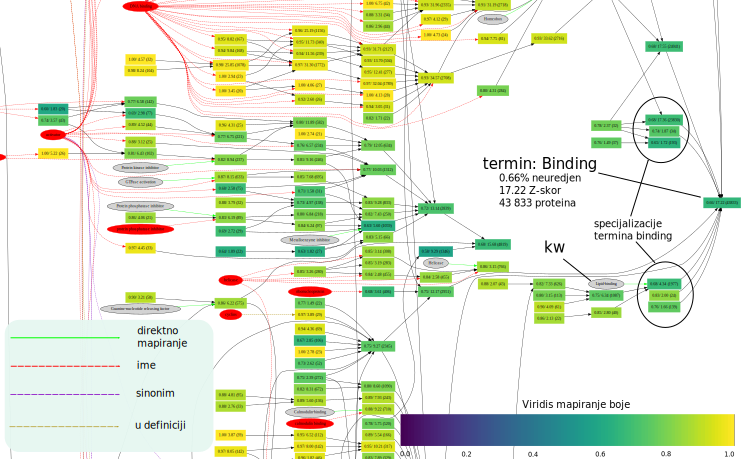
\includegraphics[ scale=0.75]{Figures/plots/disorder_example.pdf}
  \end{figure}
\end{frame}


% \subsection{Odnos prosečne dužine i p}
%
% \begin{frame}
%   \begin{figure}
%     \centering
%     \includegraphics[scale=0.86]{Figures/plots/avg_len2p.pdf}
%   \end{figure}
% \end{frame}


\subsection{Odnos neuređenosti i p}
\begin{frame}
  \begin{figure}
    \centering
    \vspace{-0.5cm}
    \includegraphics[scale=0.55]{Figures/plots/avg_dis2p.pdf}
    \caption {
      Odnos između neuređenosti (\textit{avg\_dis}) i p vrednosti MF-termina.
    }
  \end{figure}
\end{frame}


\begin{frame}
  \begin{center}
    \Huge Hvala :)
  \end{center}
\end{frame}



\end{document}
